% Temporarily as a separate document
% Will be placed inside the root latex file

\documentclass[10pt,a4paper]{article}
\usepackage[latin1]{inputenc}
\usepackage{amsmath}
\usepackage{amsthm}
\usepackage{amsfonts}
\usepackage{amssymb}
\usepackage{mathtools}
\usepackage{graphicx}
\usepackage{color}
\usepackage{hyperref}

% theorem environment
\newtheorem{prop}{Proposition}[section]
\newtheorem{theorem}{Theorem}[section]
\newtheorem{prop2}{Proposition}
\newtheorem{lem}{Lemma} 
\newtheorem{ex}{Example}

% For algorithms
\usepackage{algorithm}
\usepackage{algorithmic}

% custom commands
\newcommand{\boldvec}[1]{\boldsymbol{\mathrm{#1}}}
\let\vec\boldvec
\newcommand\at[2]{\left.#1\right|_{#2}} % the at differential sign
\newcommand\scalemath[2]{\scalebox{#1}{\mbox{\ensuremath{\displaystyle #2}}}} % scaling matrices
\DeclareMathOperator{\vect}{vec}

%% custom macros

% % % % Robot control terminology % % % %
\newcommand{\todo}{\textcolor{red}{TODO}} % TODO!
\newcommand{\kin}{\mathcal{T}} % used to denote inverse kinematics
\newcommand{\invKin}{\mathcal{T}^{-1}} % used to denote inverse kinematics

\newcommand{\joint}{\vec{q}} % used to denote robot state in joint space
\newcommand{\state}{\vec{x}} % denotes the generalized coordinates - joint space and velocity coordinates
\newcommand{\error}{\vec{e}} % difference between state and reference
\newcommand{\traj}{\vec{s}} % used to denote the points on the trajectory to be tracked

\newcommand{\dist}{\vec{\epsilon}} % denotes the disturbances acting on the rigid body dynamics
\newcommand{\linDist}{\vec{d}} % denotes the disturbances on the LTV model

\newcommand{\sysInput}{\vec{u}} % used to denote the system inputs
\newcommand{\linInput}{\tilde{\sysInput}} % denotes the LTV inputs
\newcommand{\trjInput}{\sysInput_{\mathrm{IDM}}} % denotes the inputs on the trajectory (calculated using IDM)
\newcommand{\ilcInput}{\sysInput_{\mathrm{ILC}}}

% % % % TLS terminology % % % %
\newcommand{\designMat}{\vec{X}} % design matrix
\newcommand{\observations}{\vec{y}} % observations vector
\newcommand{\param}{\vec{\beta}} % parameter vector
\newcommand{\residual}{\vec{r}} % residuals
\newcommand{\weightingMat}{\vec{W}} % weighting the residuals
\newcommand{\errorMat}{\vec{E}} % error matrix

% % % % ILC terminology % % % %
\newcommand{\qmatrix}{\vec{\Gamma}} % denotes the filtering qmatrix term of Bristow et al.
\newcommand{\lmatrix}{\vec{L}} % denotes the learning matrix of Bristow et al.
\newcommand{\systemMat}{\vec{F}} % system matrix after linearization of f
\newcommand{\dynamics}{\vec{f}}
\newcommand{\dynamicsNominal}{\dynamics_{\mathrm{nom}}}
\newcommand{\policy}{\vec{\pi}}
\newcommand{\ValueFunction}{J}
\newcommand{\episode}{k} % used for episode number

\newcommand{\totalTime}{T} % total time duration 
\newcommand{\numSteps}{N} % total number of time steps
\newcommand{\numepisode}{K} % total number of episodes

\newcommand{\threshold}{\epsilon}
\newcommand{\alg}{\emph{tILC}}
\newcommand{\dataset}{E}

\newcommand\red[1]{{\color{red}#1}}
\newcommand\blue[1]{{\color{blue}#1}}
\newcommand\bluebold[1]{\textbf{{\color{blue}#1}}}
\newcommand\gray[1]{{\color{gray}#1}}

% Set the paths where all figures are taken from:
\graphicspath{{Pictures/}}
\mathtoolsset{showonlyrefs} 
\newcommand{\includesvg}[1]{%
% \executeiffilenewer{#1.svg}{#1.pdf}%
% {inkscape -z -D --file=#1.svg %
% --export-pdf=#1.pdf --export-latex}%
 \input{#1.pdf_tex}%
}

\author{Okan Ko\c c, Guilherme Maeda and Jan Peters}
\title{Cautious Learning Control with Total Least Squares}
\begin{document}

\maketitle
\thispagestyle{empty}
\pagestyle{empty}

%%%%%%%%%%%%%%%%%%%%%%%%%%%%%%%%%%%%%%%%%%%%%%%%%%%%%%%%%%%%%%%%%%%%%%%%%%%
\begin{abstract}

Iterative Learning Control is a control theoretic learning paradigm that aims to iteratively improve the tracking performance of a repetitive system. Optimization based approaches to ILC assume that a detailed knowledge of the plant to be controlled is available. However, such approaches can diverge terribly due to overconfidence. 

In this paper, we propose a more cautious ILC algorithm using total least squares (TLS), that is robust with respect to modeling uncertainties. Moreover we give a Bayesian interpretation of TLS and build an adaptive routine that can adaptively identify the underlying linearized model. Simulation and real robot results confirm the contributions mentioned.
\end{abstract}

%%%%%%%%%%%%%%%%%%%%%%%%%%%%%%%%%%%%%%%%%%%%%%%%%%%%%%%%%%%%%%%%%%%%%%%%%%%


\section{Introduction}

% RC reference needed
Learning Control paradigms, and in particular Iterative Learning Control (ILC) \cite{Arimoto84}, \cite{Bristow06} and Repetitive Control (RC), aim to iteratively improve the tracking performance of a control system subject to repetitive tasks. In ILC, these tasks are episodic in nature: follow a desired trajectory for a fixed duration and repeat. In RC, the task is periodic but also continuous, and unlike ILC the system is not reset to a certain initial state. 

Methods that learn to track (periodic or episodic) trajectories need to compensate for modeling uncertainties and other repetitive disturbances acting on the system to be controlled. When all such disturbances are compensated for the system knowledge can be said to be indirectly acquired. However, stable methods that can efficiently and safely learn the dynamics are model-based (e.g. most of optimization-based ILC \cite{Amann95},\cite{Bristow06}) and at least require a global understanding of the dynamics of the system \cite{Kolter09}, \cite{NguyenTuong11}.

% refs needed
When executing model-based learning algorithms, it is essential for stability and safety concerns to incorporate a notion of model uncertainty. Otherwise the learning algorithms can be overconfident and easily go unstable. One way to achieve more stable performance is to use regularization. The inputs or the change in inputs applied to the system can be penalized. Such robust methods in ILC are known as Q-filtering and mostly incur a trade-off between stability and performance: system often will often converge to a nonzero steady-state error. 

In this paper, we introduce another way to increase stability margins of model-based ILC algorithms that does not incur such a trade-off. We handle the modelling uncertainty issue in a errors-in-variables regression model by using Total Least Squares (TLS) to perform the ILC updates cautiously. This way we ensure robustness with respect to model uncertainty while at the same time improving the steady-state performance. We prove that we increase the stability margin of ILC with TLS and hence ensure the monotonic convergence property of ILC for a wider range of nominal models.

To summarize, our contributions are many and can be stated as follows:

\begin{itemize}
\item We form a link between model-based Iterative Learning Control updates and errors-in-variables regression models, and analyze in particular Total Least Squares (TLS).
\item We prove that we increase the stability margins (in the iteration domain) of ILC by incorporating a truncated TLS update rule, and ensure monotonic convergence without sacrificing minimal steady-state error. 
\item We exploit the structure of the block Hankel matrix estimation problem within TLS and increase its applicability for control problems. Simulation and real robot experimental results are presented.
\item We show as an extension of our ideas, one way to incorporate a Bayesian update rule within TLS and achieve self-tuning property. 
\end{itemize}

The outline of the paper is as follows: in the next subsection \ref{relatedWork} we give a brief literature review related to our work. In section \ref{methodology} we start by analyzing Total Least Squares. We present truncated structured TLS, along with pseudocode, and show its applicability in Iterative Learning Control. The resulting algorithm $\alg$ with minor modifications can be applied to Repetitive Control (RC) as well. In subsection \ref{ilcTLS} we prove the monotonic convergence and minimal steady state error of $\alg$. An adaptive version of $\alg$ is presented in \ref{adaptiveILC}, simulation results and real robot experiments are given in \ref{results}. Finally, conclusions and brief mention of possible future directions to explore are given in \ref{conclusions}.

% references required as always.  
\subsection{Related Work}\label{relatedWork}

A thorough investigation of the statistical properties of Total Least Squares (TLS) as well as its extensions such as structured TLS is presented in \cite{VanHuffel91}. For a short overview see \cite{Golub80} or \cite{Golub96}. Literature on TLS is huge and the application areas are growing rapidly. For some of the applications of TLS and errors-in-variables modelling, see the recent book \cite{VanHuffel13}.

One of the first papers that introduced Iterative Learning Control (ILC) is \cite{Arimoto84}. For a good survey, see \cite{Bristow06} or \cite{Moore07}. Desirable properties of ILC algorithms include stability and monotonicity, and are discussed, for example, in \cite{Norrloef02}. Optimization based ILC is described, for example, in \cite{Amann95}, \cite{Bristow06}, \cite{Moore07}. It seems we are not the first to notice the connection between ILC and TLS: another application of TLS in ILC is given in \cite{ZhangBo14}.

% % 2D systems analysis reference?
% % More applications of TLS? Especially in system identification, modelling, signal processing, etc.
% % Repetitive Control??

\section{Methodology}\label{methodology}
%
\subsection{Linear Least Squares}
Let $\designMat \in \mathbb{R}^{m \times n}$ be the design matrix, $\observations \in \mathbb{R}^{m}$ the vector of observations and  $\param \in \mathbb{R}^{n}$ the parameter vector to be estimated: $\designMat\param \approx \observations$. In this linear regression model $\residual = \observations - \designMat\param$ are the residuals that are to be minimized with respect to 2-norm
%
\begin{equation}
\begin{aligned}
\text{minimize} &\ \residual^{\mathrm{T}}\weightingMat\residual, \\
\text{subject to} &\ \observations + \residual \in \text{Range}(\designMat).
\end{aligned}
\end{equation}
%

\subsection{Total Least Squares: an errors-in-variables model}

Total Least Squres (TLS) is an errors-in-variables model that is applicable when the design matrix is also not precise
$(\designMat + \errorMat)\param = \observations + \residual$. An optimization procedure under this model with no weighting is as follows
%
\begin{equation}
\begin{aligned}
\text{minimize} &\ \|\begin{bmatrix} \errorMat & \residual \end{bmatrix}\|_{F} \\
\text{subject to} &\ \observations + \residual \in \text{Range}(\designMat + \errorMat)
\end{aligned}
\end{equation}
%
In general TLS fails to have a closed form solution. An example with low-rank design matrix can be found in \cite{Golub80}. % when is it guaranteed to have a closed form solution? What about truncated TLS??

%\begin{equation}
%\begin{aligned}
%\designMat = \begin{bmatrix}
%   1 & 0 \\ 0 & 0
% \end{bmatrix}, \ Y = \begin{bmatrix}
% 1 \\ 1
% \end{bmatrix} 
%\end{aligned}
%\end{equation}
%For every $\epsilon > 0$, $Y \in \text{Range}(\designMat + E_{\epsilon}), \ E_{\epsilon} = \begin{bmatrix} 0 & 0 \\ 0 & \epsilon \end{bmatrix}$


An SVD Solution to TLS is also described in \cite{Golub80}. Rewriting $(\designMat + \errorMat)\param = \observations + \residual$ as  
%
\begin{equation}
\begin{aligned}
\begin{bmatrix} \designMat + \errorMat & \observations + \residual \end{bmatrix} \begin{bmatrix} \param \\ -1 \end{bmatrix} = 0 \\
\end{aligned}
\end{equation}
%
and using the Eckart-Young theorem
\begin{equation}
\begin{aligned}
\begin{bmatrix} \designMat & \observations \end{bmatrix} = \begin{bmatrix} U_{\designMat} & U_{\observations} \end{bmatrix} \begin{bmatrix} \Sigma_{\designMat} & 0 \\ 0 & \Sigma_{\observations} \end{bmatrix} \begin{bmatrix} V_{\designMat \designMat} & V_{\designMat \observations} \\ V_{\observations \designMat} & V_{\observations \observations} \end{bmatrix}^{\mathrm{T}} \\
\begin{bmatrix} \designMat + \errorMat & \observations + \residual \end{bmatrix} = \begin{bmatrix} U_{\designMat} & U_{\observations} \end{bmatrix} \begin{bmatrix} \Sigma_{\designMat} & 0 \\ 0 & 0 \end{bmatrix} \begin{bmatrix} V_{\designMat \designMat} & V_{\designMat \observations} \\ V_{\observations \designMat} & V_{\observations \observations} \end{bmatrix}^{\mathrm{T}}
\end{aligned}
\end{equation}
% 
After subtracting and manipulating we get
%
\begin{equation}
\begin{aligned}
\hat{\param}_{tls} &= -V_{\designMat \observations}V_{\observations \observations}^{-1} \\
\hat{\errorMat} &= U_{\designMat} \Sigma_{\designMat} V_{\designMat \designMat}^{\mathrm{T}} - \designMat
\end{aligned}
\end{equation}

Many extensions are available: global, structured, truncated. % citation necessary!
Truncated total least squares (TTLS) can be written simply as
%
\begin{equation}
\begin{aligned}
\hat{\param}_{ttls} = -V_{\designMat \observations}V_{\observations \observations}^{\dagger}
\end{aligned}
\end{equation}
%

\begin{figure}
\centering
\includegraphics[width=0.4\textwidth]{LSvsTLS.jpg}%
\caption{Total Least Squares minimizes in 1D the sum of the squared perpendicular distances.}
\end{figure}
%
\subsection{Iterative Learning Control with Total Least Squares}\label{ilcTLS}
%
Linearize nominal robot dynamics $\dot{\state} = \dynamicsNominal(\state,\sysInput)$ around a fixed trajectory $\traj$ to predict the errors incurred along the trajectory $\error = \state - \traj$
%
\begin{equation}
\begin{aligned}
\error \approx \systemMat \sysInput - \linDist.
\end{aligned}
\end{equation}
%
ILC using this model computes at every iteration the feedforward compensation signal $\sysInput$ to drive error $\error$ to $\vec{0}$. For example, a pseudo-inverse based ILC computes the updates using
%
\begin{equation}
\begin{aligned}
\sysInput = \systemMat^{\dagger}\linDist.
\end{aligned}
\end{equation}
%
However robot dynamics may not be known well! We take this into account by using truncated Total Least Squares to come up with a more cautious ILC update
%
\begin{equation}
\begin{aligned}
\sysInput_{TLS}, \ \errorMat &= \arg\min_{\sysInput,\errorMat} \|\begin{bmatrix}\errorMat & \residual \end{bmatrix} \|_{F}, \\
\residual &= \linDist - (\systemMat + \errorMat)\sysInput.
\end{aligned}
\end{equation}
%
\subsection{Adaptive ILC based on Bayesian TLS}\label{adaptiveILC}
%
% The prior weighting of the nominal model before starting the adaptive procedure can be based on the number of samples used in the identification of the block Hankel matrix F.

% Bayesian ILC is by definition a higher order ILC!

\section{Results}\label{results}

%
\subsection{Simulation Results of Seven DOF Barrett Arm}
%
In the simulation results shown below, ILC with pseudoinverse cannot approach trajectory very well, and after 8 iterations starts to diverge.
\begin{figure}
\centering
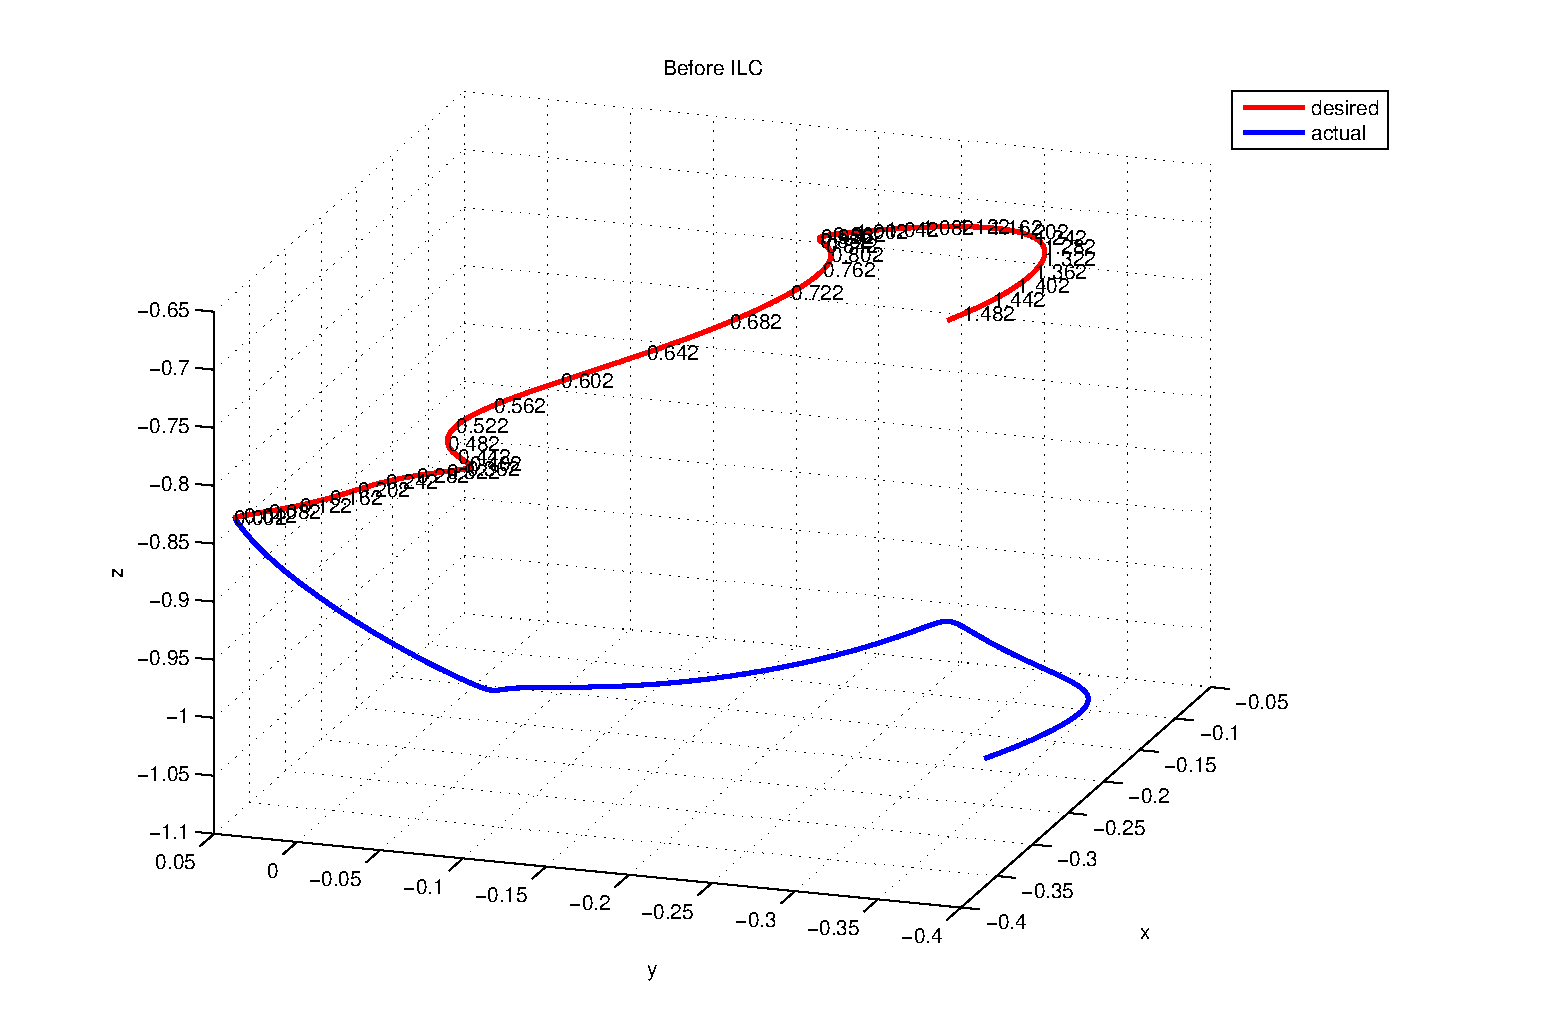
\includegraphics[width=0.5\textwidth]{beforeILC.eps}%
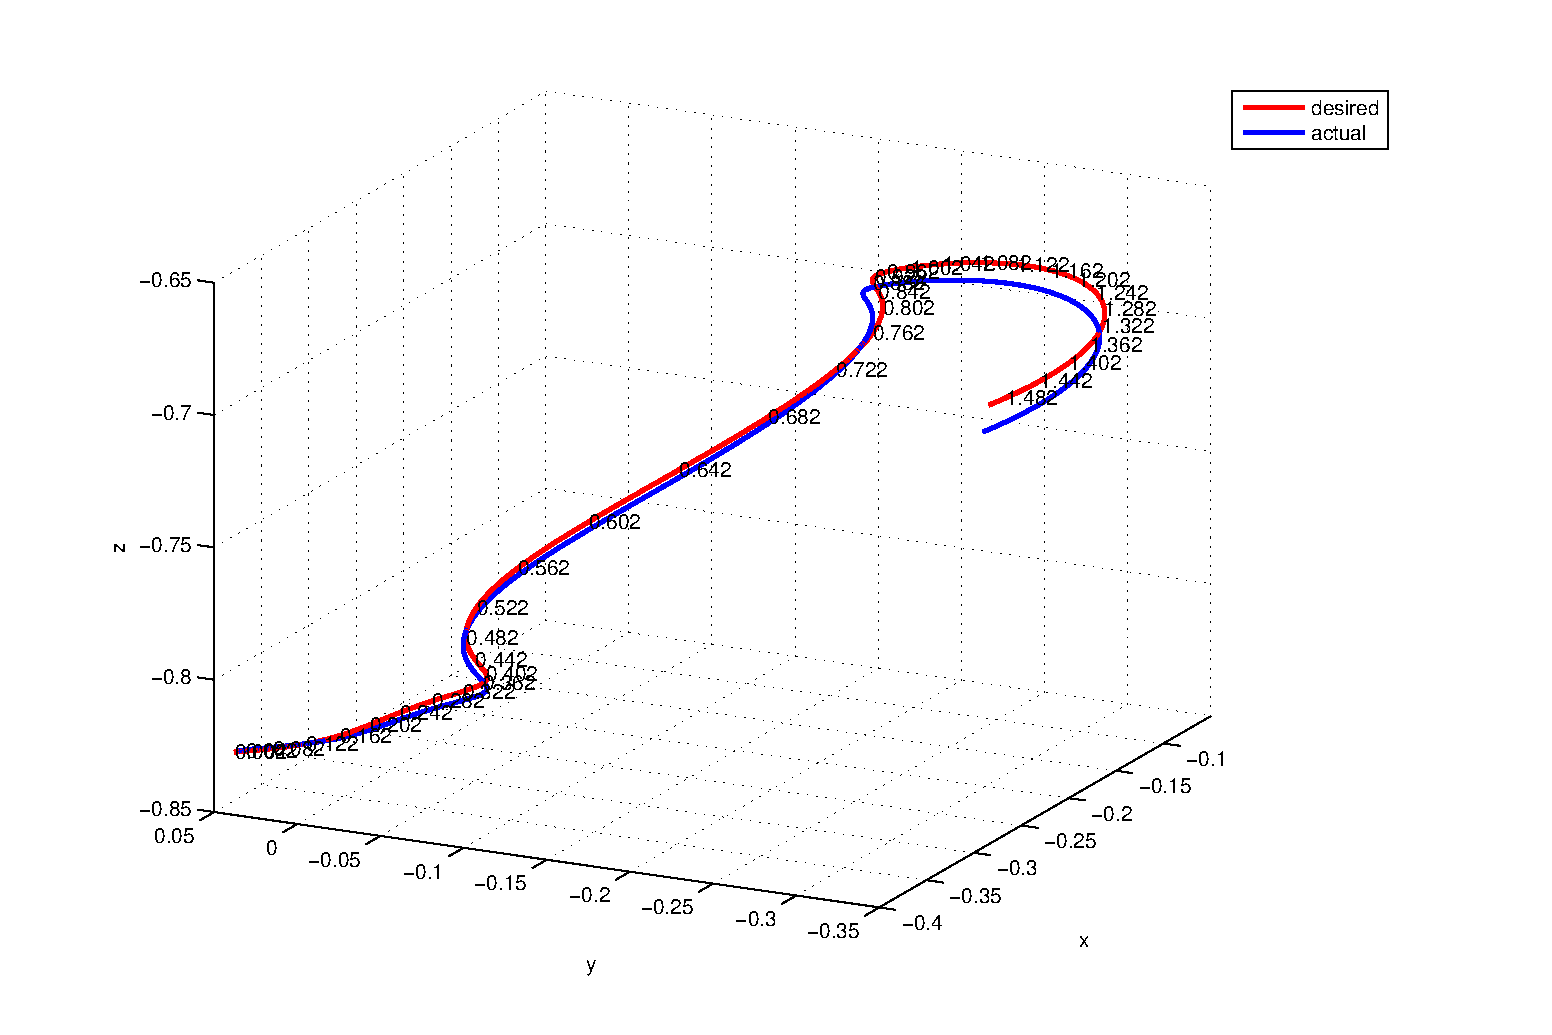
\includegraphics[width=0.5\textwidth]{afterILCPseudoInv.eps}		
\caption{Before and after applying ILC (10 iterations)}
\end{figure}
%
ILC with truncated total least squares on the other hand approaches the trajectory very well, and shows excellent tracking performance.
%
\begin{figure}
\centering
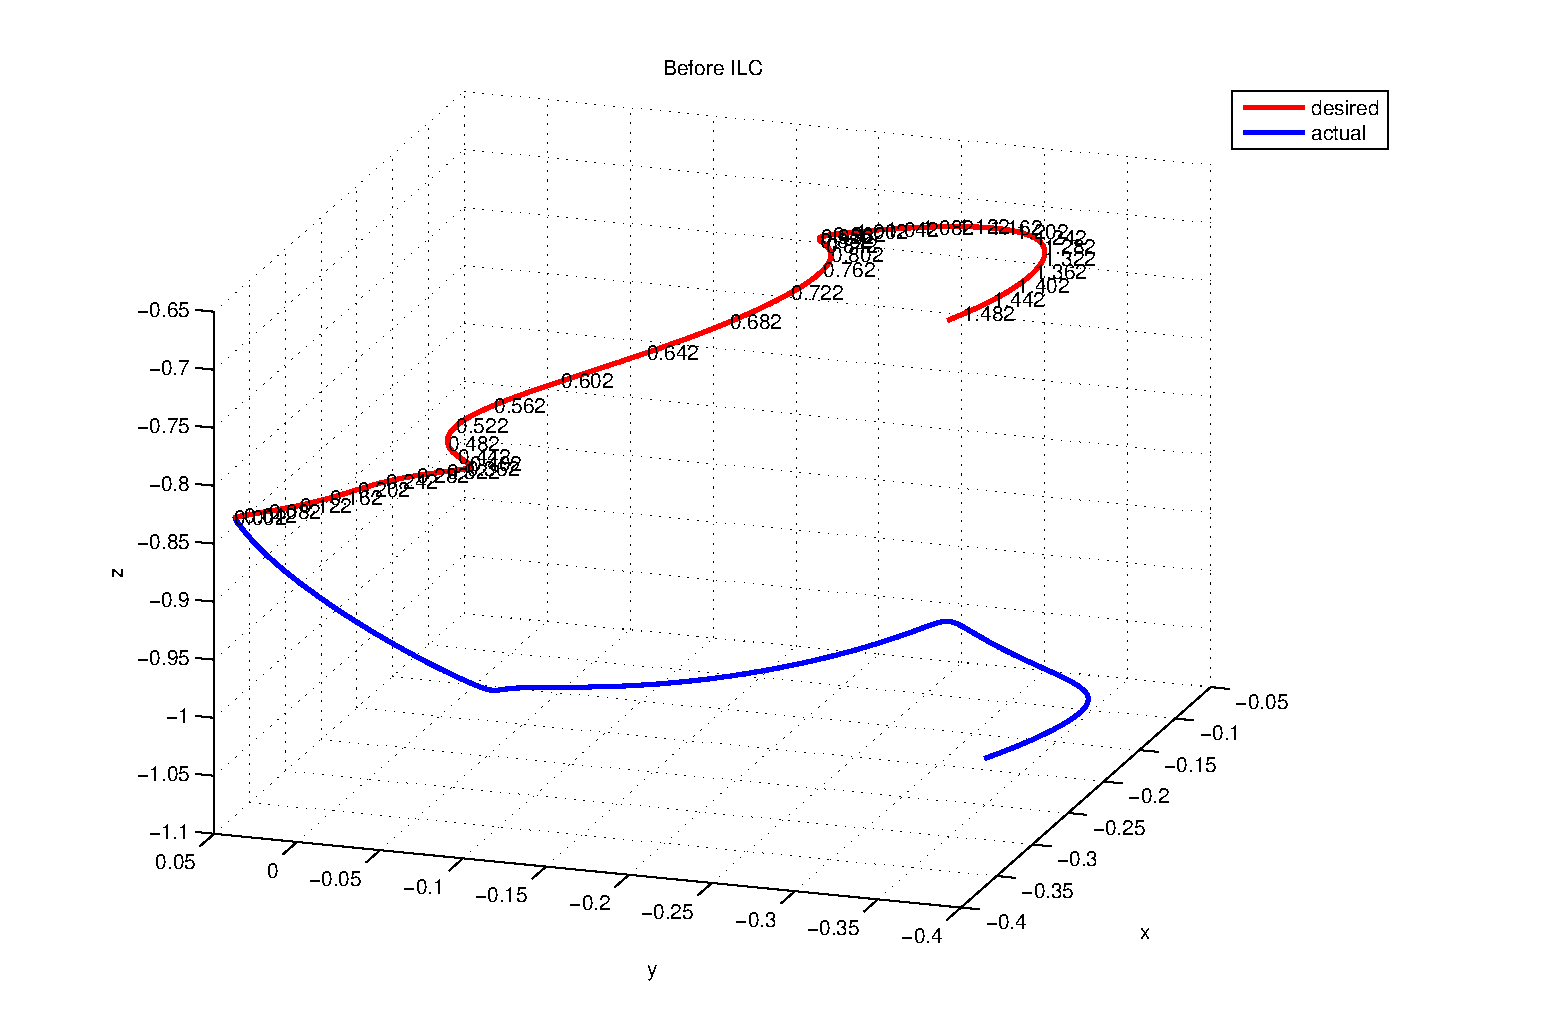
\includegraphics[width=0.5\textwidth]{beforeILC.eps}%
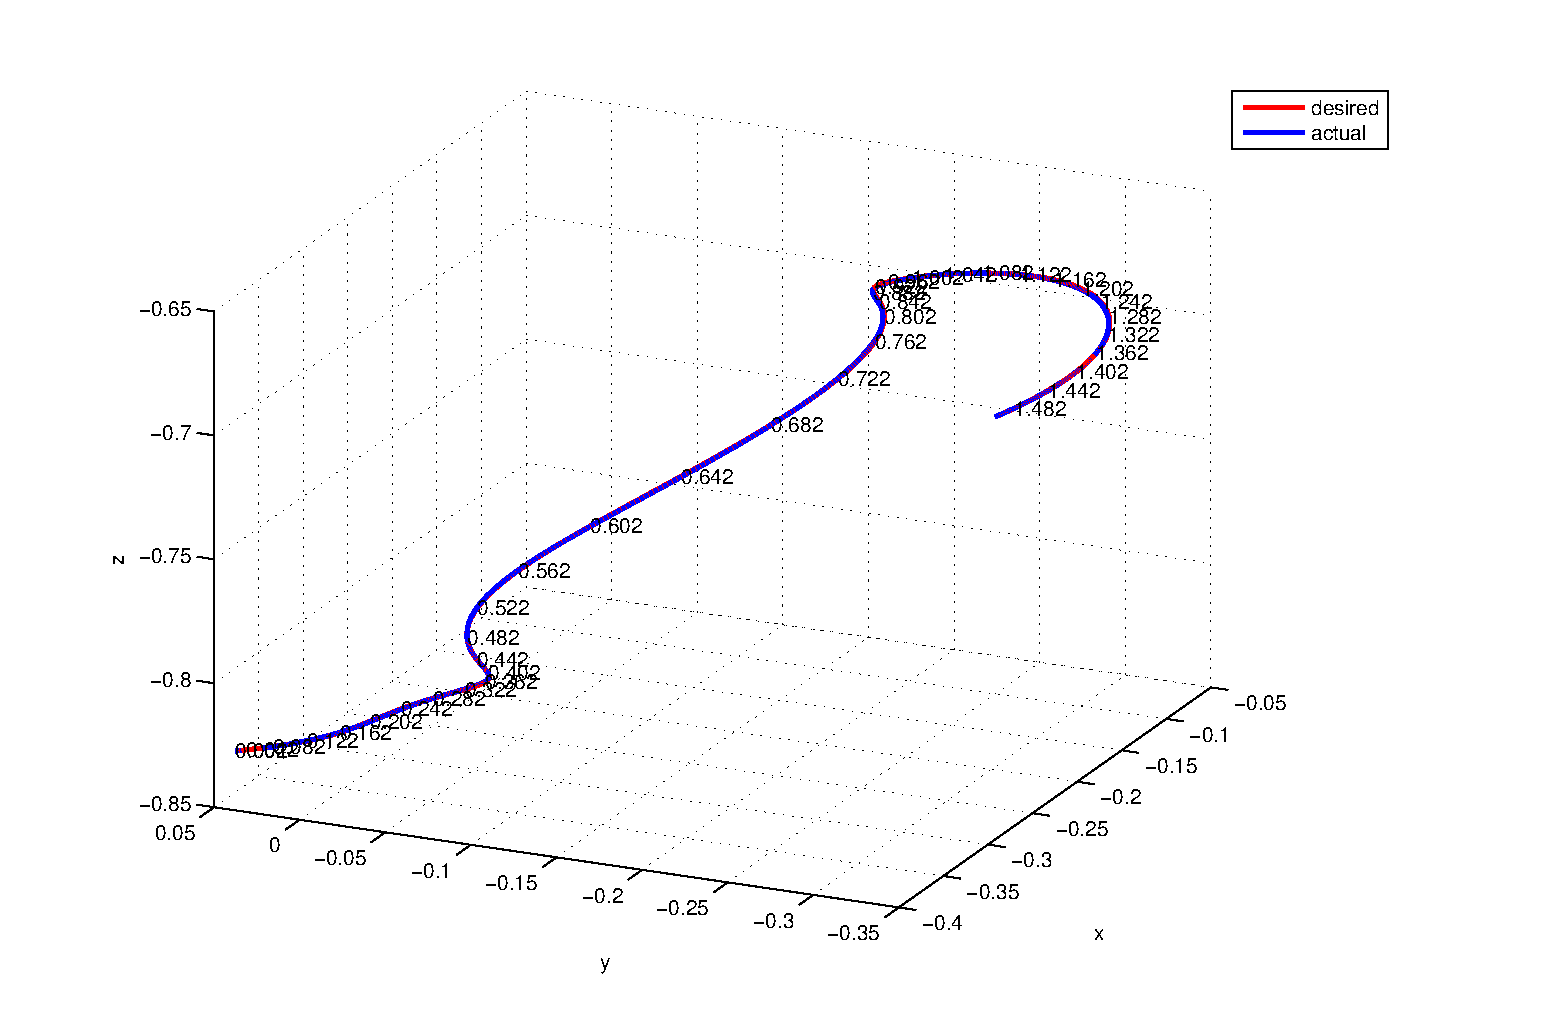
\includegraphics[width=0.5\textwidth]{afterILCTLS.eps}		
\caption{Before and after applying ILC (10 iterations)}
\end{figure}
%

\subsection{Applications in Robotic Table Tennis}

\section{Conclusions and Future Work}\label{conclusions}


\bibliographystyle{plain}
%\bibliographystyle{./IEEEtran}
%\bibliography{./IEEEabrv,./iros2015Ref}
\bibliography{./tempRef}

\end{document}
